\section{Jets}
\label{sec:jets}

Due to the confining nature of QCD, color-charged quarks and gluons produced in the
initial $pp$ interactions do not exist as free states for observably meaningful
timescales and therefore do not leave unambiguous signatures in the detector.
Instead, their production is characterised by the radiation of additional
quarks and gluons roughly collinear with the initiating colored particles.
The radiation pattern of these colored objects is dictated by the color field
that binds them and eventually results in the production of color-neutral hadrons.
The collimated spray of hadrons as a result of this \textit{hadronisation} process
leads to the phenomenology of \textit{jets}, which are the macroscopically observable signature
of produced quarks and gluons.
The reconstruction of jets refers to any suitable, i.e. physically meaningful and stable,
method for grouping together, or \textit{clustering}, the end-products of the hadronisation
process in such a way that the properites of the initiating quarks or gluons, such
as their quantum numbers and/or kinematics, can be inferred from the resulting clustered object.
The standard method for reconstructing jets in ATLAS will be introduced in Section~\ref{sec:jet_reco}.
In Section~\ref{sec:jet_calib}, the steps taken to turn these reconstructed jets into
accurate representations of the initiating quarks and/or gluons, so that they can
be used meaningfully in physics analyses, will be discussed.

\begin{figure}[!htb]
    \begin{center}
        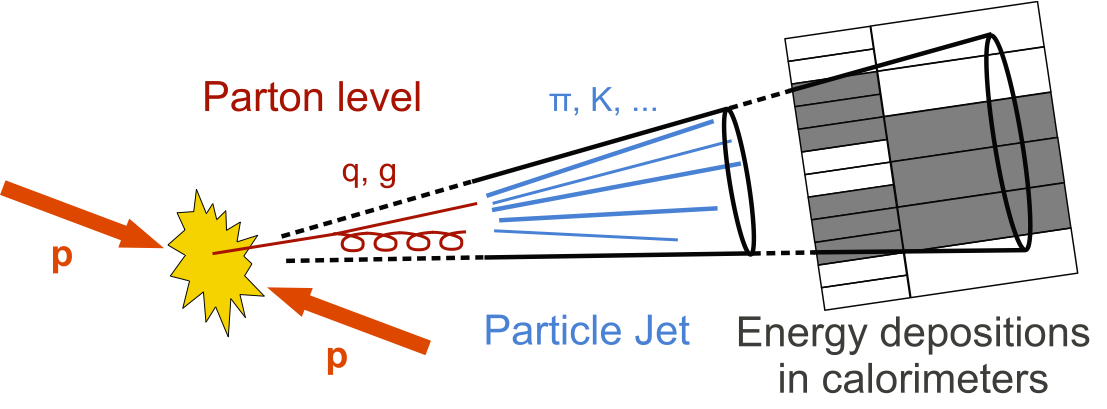
\includegraphics[width=0.7\textwidth]{figures/chapter3/jets/jet_formation_cartoon}
        \caption{
            Illustration of the jet formation process, beginning with the initiating quark and/or
            gluons (partons) which hadronise to form particle jets discernible by the tracking detectors
            in the ID and calorimeter jets defined by energy depositions in the calorimeter systems.
        }
        \label{fig:jet_formation}
    \end{center}
\end{figure}

\FloatBarrier
\subsection{Jet Reconstruction}
\label{sec:jet_reco}

\subsubsection{Topological Cell Clustering}
\label{sec:jet_topo_cluster}

The process of jet reconstruction begins first with the clustering of the lowest level calorimeter elements,
\textit{calorimeter cells}, corresponding to the readout channels in the LAr and tile calorimeters.
Figure~\ref{fig:calocell_granularity} gives an idea of the calorimeter cell granularity across the calorimeter
system.
The clustering algorithm used by ATLAS is a three-dimensional \textit{topological clustering} algorithm~\cite{Lampl:2008zz,Aad:2016upy}.
The highly granular calorimeter system used in ATLAS, with its finely segmented lateral readout and longitudinal sampling layers,
allows for the subsequent topological clusters (`topo-clusters') to capture in detail the energy-flow details of jets.
Topo-cluster formation begins by first identifying so-called \textit{seed cells} which have a rather high signal-to-noise ratio ($S/N$),
$S/N>4$.
Here, the signal is defined as the absolute value of the calorimter-cell energy measurement, $\lvert E \rvert$,
and the noise is defined as the sum in quadrature of the RMS of the electronics and expected pileup noise contributions.
Cells neighboring the seed cells satisfying $S/N>2$ are then collected into the topo-cluster.
A neighboring cell is defined in three-dimensions as either the calorimeter cells directly adjacent within the same calorimeter layer as
the seed cell, or, if in adjacent layers or in different calorimeter sub-systems, cells having at least partial overlap
in the $(\eta,\phi)$ plane with the seed.
The final set of cells, the perimeter cells, satisfying $S/N\ge0$ are then collected.
This last threshold essentially collects all those cells surrounding already-collected cells within each layer.
Figure~\ref{fig:calocell_clustering} illustrates the concept of topological cell clustering as described here.

\begin{figure}[!htb]
    \begin{center}
        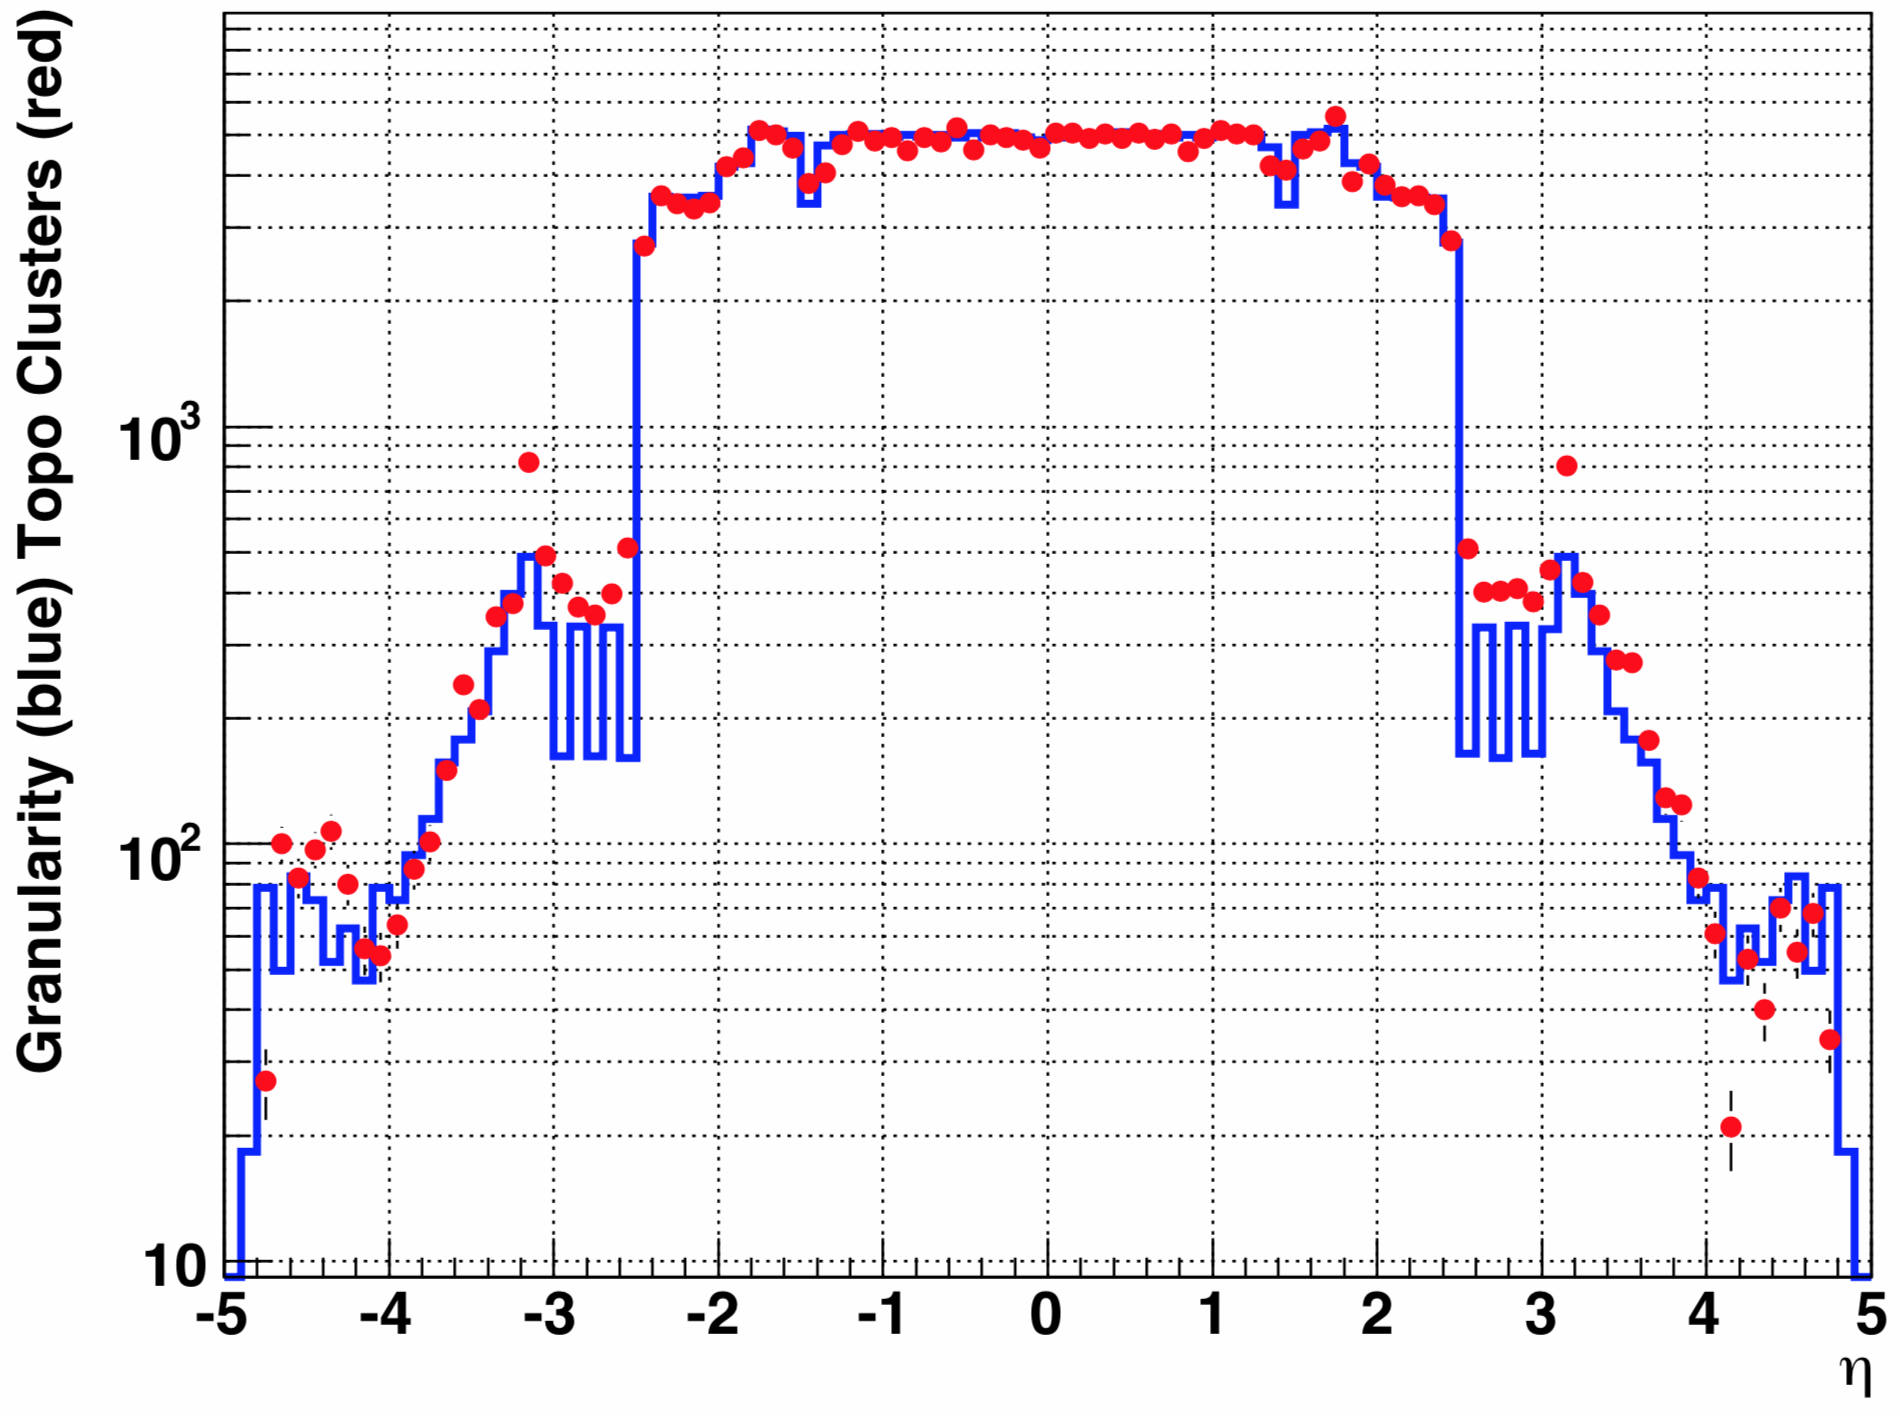
\includegraphics[width=0.5\textwidth]{figures/chapter3/jets/calocell_granularity}
        \caption{
            The blue histogram shows the average calorimeter cell granularity, i.e. number of calorimeter cells per
            $\Delta \eta = 0.1$, as a function of detector $\eta$. The red points show an approximation of the blue
            histogram based on calculations of the expected noise per calorimeter cell.
            From Ref.~\cite{Lampl:2008zz}.
        }
        \label{fig:calocell_granularity}
    \end{center}
\end{figure}

\begin{figure}[!htb]
    \begin{center}
    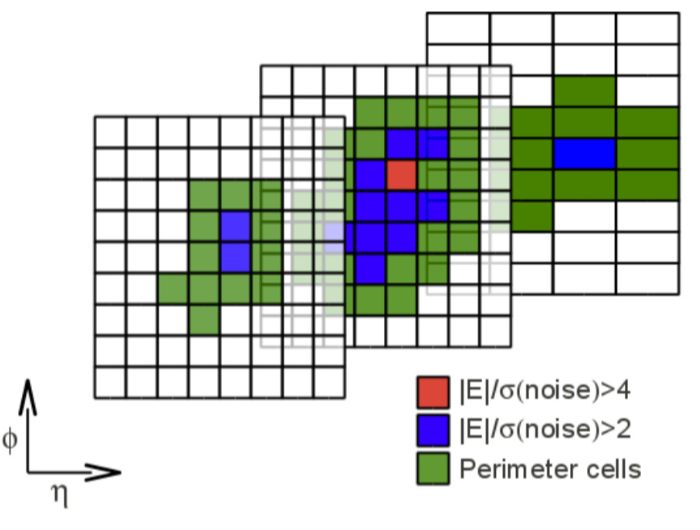
\includegraphics[width=0.6\textwidth]{figures/chapter3/jets/calocell_clustering_cartoon}
    \caption{
        Illustration of calorimeter-cell topological clustering across the three layers of the
        hadronic calorimeter. Indicated are the cells satisfying the signal-to-noise requirements for
        the seed (red), neighbor (blue), and perimeter (green) cells that make up the final three-dimensional topo-cluster.
    }
    \label{fig:calocell_clustering}
    \end{center}
\end{figure}
\FloatBarrier

\subsubsection{Jet Finding}
\label{sec:jet_finding}

Once the set of topo-clusters is formed, the process of jet finding begins.
As there is no single unique way to define a jet, there is a wide variety of jet finding algorithms whose
purpose is to associate jet constituents --- here, the calorimeter-cell topo-clusters --- to form
the final object representing the jet.
The default jet finding algorithm used by ATLAS is the
\textit{\antikt} jet clustering algorithm~\cite{Cacciari:2008gp}.
The \antikt~algorithm belongs to the more general class of sequential recombination algorithms
and is favored for its infrared and collinear (IRC) safe properties as well as the fact
that it tends to produce rather simple jets, geometrically, that are circular in the $\eta-\phi$ plane,
as seen in Figure~\ref{fig:antikt_circles}.
IRC safety in jet finding algorithms refers to the property that neither additional collinear splitting of jet constituents (e.g. the initiating or radiated partons)
nor soft emissions should change the clustered jet.
IRC-safe jets are therefore robust against these divergent regimes of QCD, sensitive to arbitrary
calculational choices made in perturbation theory, and makes them physically  meaningful observable objects
with which one can make predictions.

The \antikt algorithm takes as input constituents the topo-clusters described in Section~\ref{sec:jet_topo_cluster}
and computes the quantities,
\begin{align}
        d_{ij} = \min \left( \frac{1}{k^2_{T,i}} , \frac{1}{k^2_{T,j}} \right) \frac{ \Delta R_{ij}^2}{R^2},
        \label{eq:antikt_0}
\end{align}
\begin{align}
        d_{iB} = \frac{1}{k_{T,i}^2},
        \label{eq:antikt_1}
\end{align}
with $\Delta R_{ij}^2 = (\eta_i - \eta_j)^2 + (\phi_i - \phi_j)^2$, {\color{red}{its rapidity, right?}} $R$ is a parameter whose value regulates the radial extent of
the jet, and $k_{T,i}$ is the transverse momentum of the $i^{th}$ constituent.
The $d_{ij}$ and $d_{iB}$ quantities are `distance' metrics used in the clustering of input topo-cluster constituents.
The former represents the `distance' between the $i^{th}$ and $j^{th}$ constituent while latter represents the
`distance' between the $i^{th}$ consituent and the beam-line, introduced to distinguish between constituents
originating from the primary hard-scatter vertex and those originating from soft proton interaction remnants.
The work to be discussed in the present thesis sets $R=0.4$, which is the standard used in ATLAS.

The \antikt algorithm proceeds by clustering those constituents whose inter-distance is smallest, thereby tending to cluster
higher-\pT constituents together, which can be seen by inspection of Equation~\ref{eq:antikt_0} and \ref{eq:antikt_1}.
If, of the set of input constituents, the smallest distance is a $d_{ij}$, the associated constituents indicated by $i$
and $j$ are recombined to form a single constituent in the list that replaces them both.
If the smallest distance is a $d_{iB}$, then the constituent indicated by index $i$ is removed from the set of constituents
and is considered as a complete jet.
This process repeats, starting with the now smaller (due to successful constituent recombination or removal) set of constituents,
until no constituents are left.
The result of this process is a set of recombined constituents that represent jets, as illustrated in Figure~\ref{fig:antikt_circles}.

\begin{figure}[!htb]
    \begin{center}
        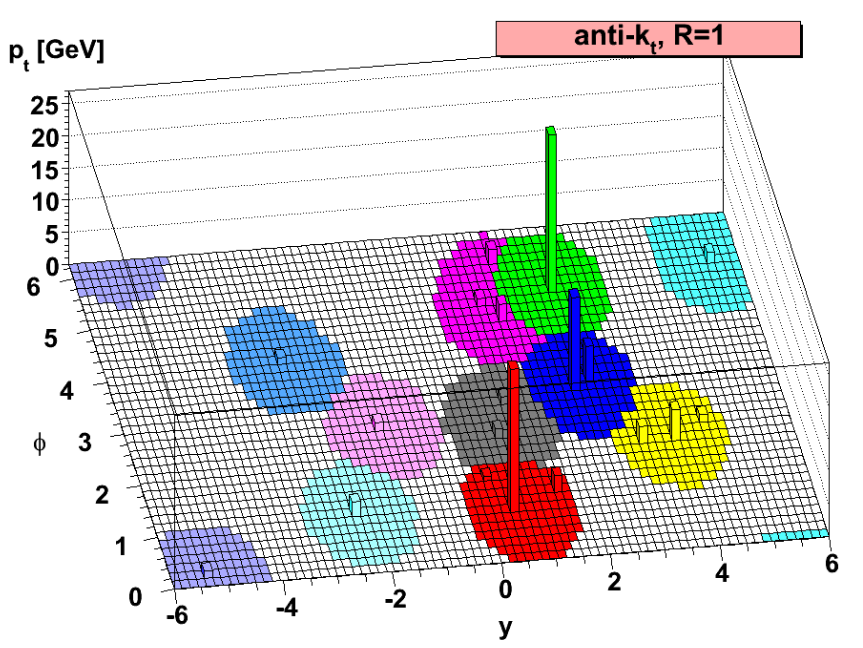
\includegraphics[width=0.5\textwidth]{figures/chapter3/jets/antikt_jet_circles}
        \caption{
            An illustration of jet constituents clustered by the \antikt~algorithm. Seen
            are the energetic constituents.
            The filled and colored circles represent areas populated by soft jet consituents, and represent the jet \textit{catchment area}~\cite{Cacciari:2008gn}
            whose size is dictated by the $R$ parameter in the \antikt algorithm (Equation~\ref{eq:antikt_0}).
            Figure taken from Ref.~\cite{Cacciari:2008gp}.
        }
        \label{fig:antikt_circles}
    \end{center}
\end{figure}

\FloatBarrier
%%%%%%%%%%%%%%%%%%%%%%%%%%%%%%%%%%%%%%%%%%%%%%%%%%%%%%%%%%%%%%%%%%%%%%%%%%%%%%%%%%%%%%%%%%%%%%%%%%
%%%%%%%%%%%%%%%%%%%%%%%%%%%%%%%%%%%%%%%%%%%%%%%%%%%%%%%%%%%%%%%%%%%%%%%%%%%%%%%%%%%%%%%%%%%%%%%%%%
%
% CALIBRATION
%
%%%%%%%%%%%%%%%%%%%%%%%%%%%%%%%%%%%%%%%%%%%%%%%%%%%%%%%%%%%%%%%%%%%%%%%%%%%%%%%%%%%%%%%%%%%%%%%%%%
%%%%%%%%%%%%%%%%%%%%%%%%%%%%%%%%%%%%%%%%%%%%%%%%%%%%%%%%%%%%%%%%%%%%%%%%%%%%%%%%%%%%%%%%%%%%%%%%%%


\subsection{Jet Calibration}
\label{sec:jet_calib}

\begin{figure}[!htb]
    \begin{center}
        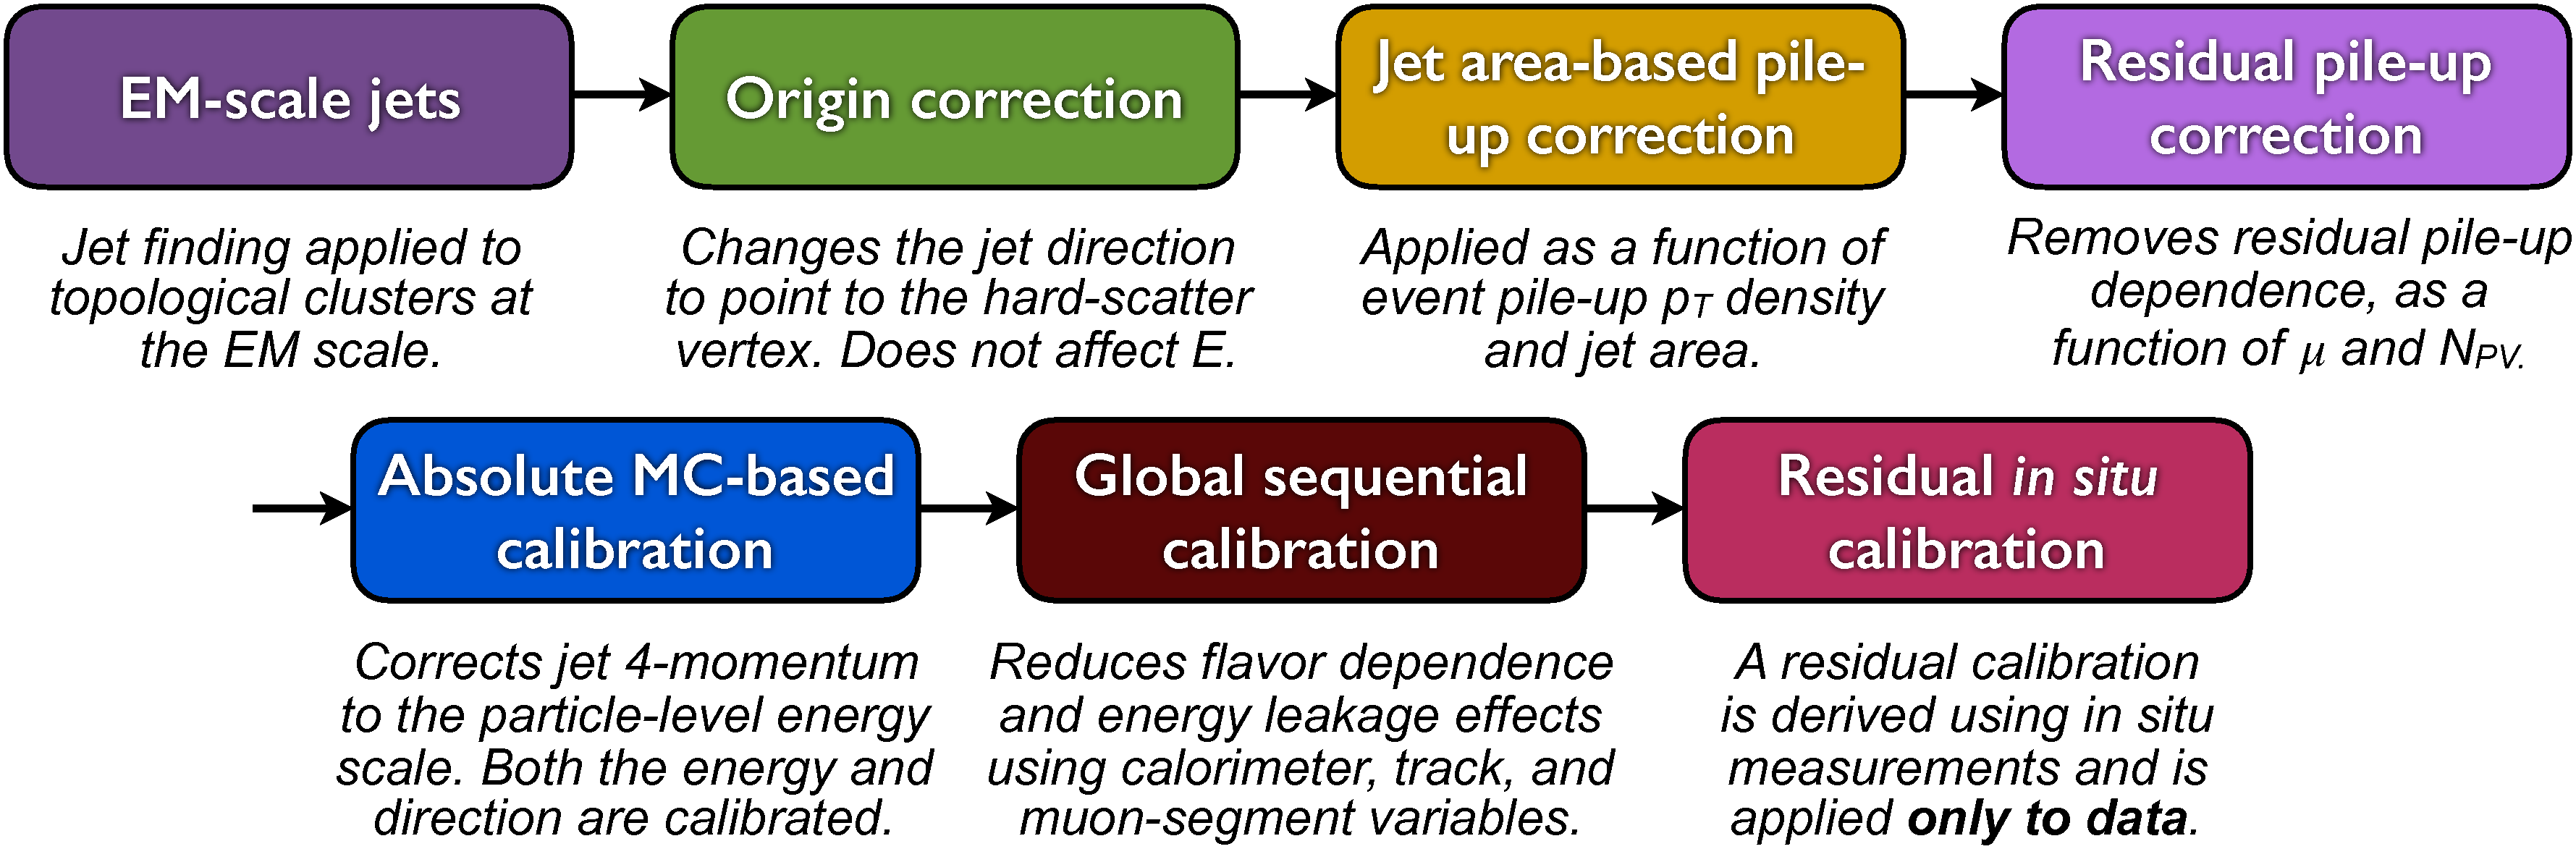
\includegraphics[width=0.8\textwidth]{figures/chapter3/jets/jes_calibration_sequence}
        \caption{
            From Ref.~\cite{Aaboud:2017jcu}.
        }
        \label{fig:jes_sequence}
    \end{center}
\end{figure}

The jets reconstructed following the steps described in Section~\ref{sec:jet_reco} are objects clustered
at the electromagnetic (EM) scale, which correctly measures the energy of electromagnetic showers but does not
accurately account for energy depositions arising as a result of hadronic shower growths.
These jets are therefore referred to as `EM-scale' jets.
To correctly assign meaningful energy and momentum measurements to the reconstructed jets that correspond
to the energies and momenta of the initiating, underlying particle-level jets, several \textit{jet energy scale} (JES) calibration steps are taken~\cite{Aaboud:2017jcu}.
The steps are detailed in the flowchart in Figure~\ref{fig:jes_sequence} and will be briefly described in the following text.

\subsubsection{Jet Origin Correction}
\label{sec:jet_origin_correction}

The reconstructed EM-scale jets are built with the assumption that they originate from the geometric center
of the detector, as opposed to the primary hard-scatter vertex from which the initiating partons arise.
The so-called jet origin corretion, therefore, refers to recalculating the jet four-momentum vector by adjusting it
in such a way that it points to the primary hard-scatter vertex.
This correction acts primarily to improve the $\eta$ resolution of jets.
This procedure is only one hundred percent accurate, of course, under the assumption that all of the jet constituents
going into the EM-scale jet reconstruction originated from the hard-scatter vertex, as opposed to some fraction having come from
a pileup vertex, for example.

\subsubsection{Pileup Corrections}
\label{sec:jet_pileup_correction}

Jets are extended object with relatively large \textit{catchment areas}~\cite{Cacciari:2008gn} that make them susceptible to
pileup effects.
Several corrections, therefore, to the jet energy are taken in order to account for contributions to the EM-scale jet reconstruction
arising from both in-time and out-of-time pileup interactions.

The first pileup correction is an area-based correction which subtracts the per-event pileup contribution to the
\pT~of each jet based on the jet's area, where the jet area is defined as in Ref.~\cite{Cacciari:2008gn}.
This pileup contribution is taken as the median \pT~density, $\rho$, of jets in the $\eta-\phi$ plane and
can be thought of as a baseline `noise' term contributing to a jet's reconstructed energy.
The quantity $\rho$ depends on the pileup activity in the event and is taken as a function of the number of reconstructed
primary vertices (\npv) in a given event; for example, the pileup density is expected to be larger for an event
with $\npv = 25$ as compared to one with $\npv = 5$.

After the area-based pileup correction is made, there still remains residual dependence of the reconstructed jet \pT~on the
number of reconstructed primary vertices and on the number of interactions, $\mu$.
These dependences are measured by performing linear fits of the jet \pT~as a function of each quantity, binned as a function of the detector $\eta$, $\eta_{\text{det}}$.

The final, pileup-corrected jet \pT~is given by Equation~\ref{eq:jet_pileup_corr}:
\begin{align}
    \pT^{\text{Corr}} = \pT^{\text{Reco}} - \underbrace{\rho \times A}_{\text{Area-based}} - \underbrace{\alpha \times (\npv - 1) - \beta \times \mu}_{\text{Residual}},
    \label{eq:jet_pileup_corr}
\end{align}
where $A$ is the jet area, and the $\alpha$ and $\beta$ terms are derived from the linear fits mentioned above and are $\alpha = \partial \pT / \partial \npv$
and $\beta = \partial \pT / \partial \mu$, respectively.
The former accounts for effects arising as a result of in-time pileup and the latter for those due to out-of-time pileup.
The effect of the pileup corrections is shown in Figure~\ref{fig:jet_pileup_corr}, where it can be seen that the area-based correction
is an overall offset, as expected, and the residual corrections have a dependence on $\lvert \eta_{\text{det}} \rvert$.
The residual pileup dependence being largest in the forward regions of the detector where pileup and background activity is largest.

\begin{figure}[!htb]
    \begin{center}
        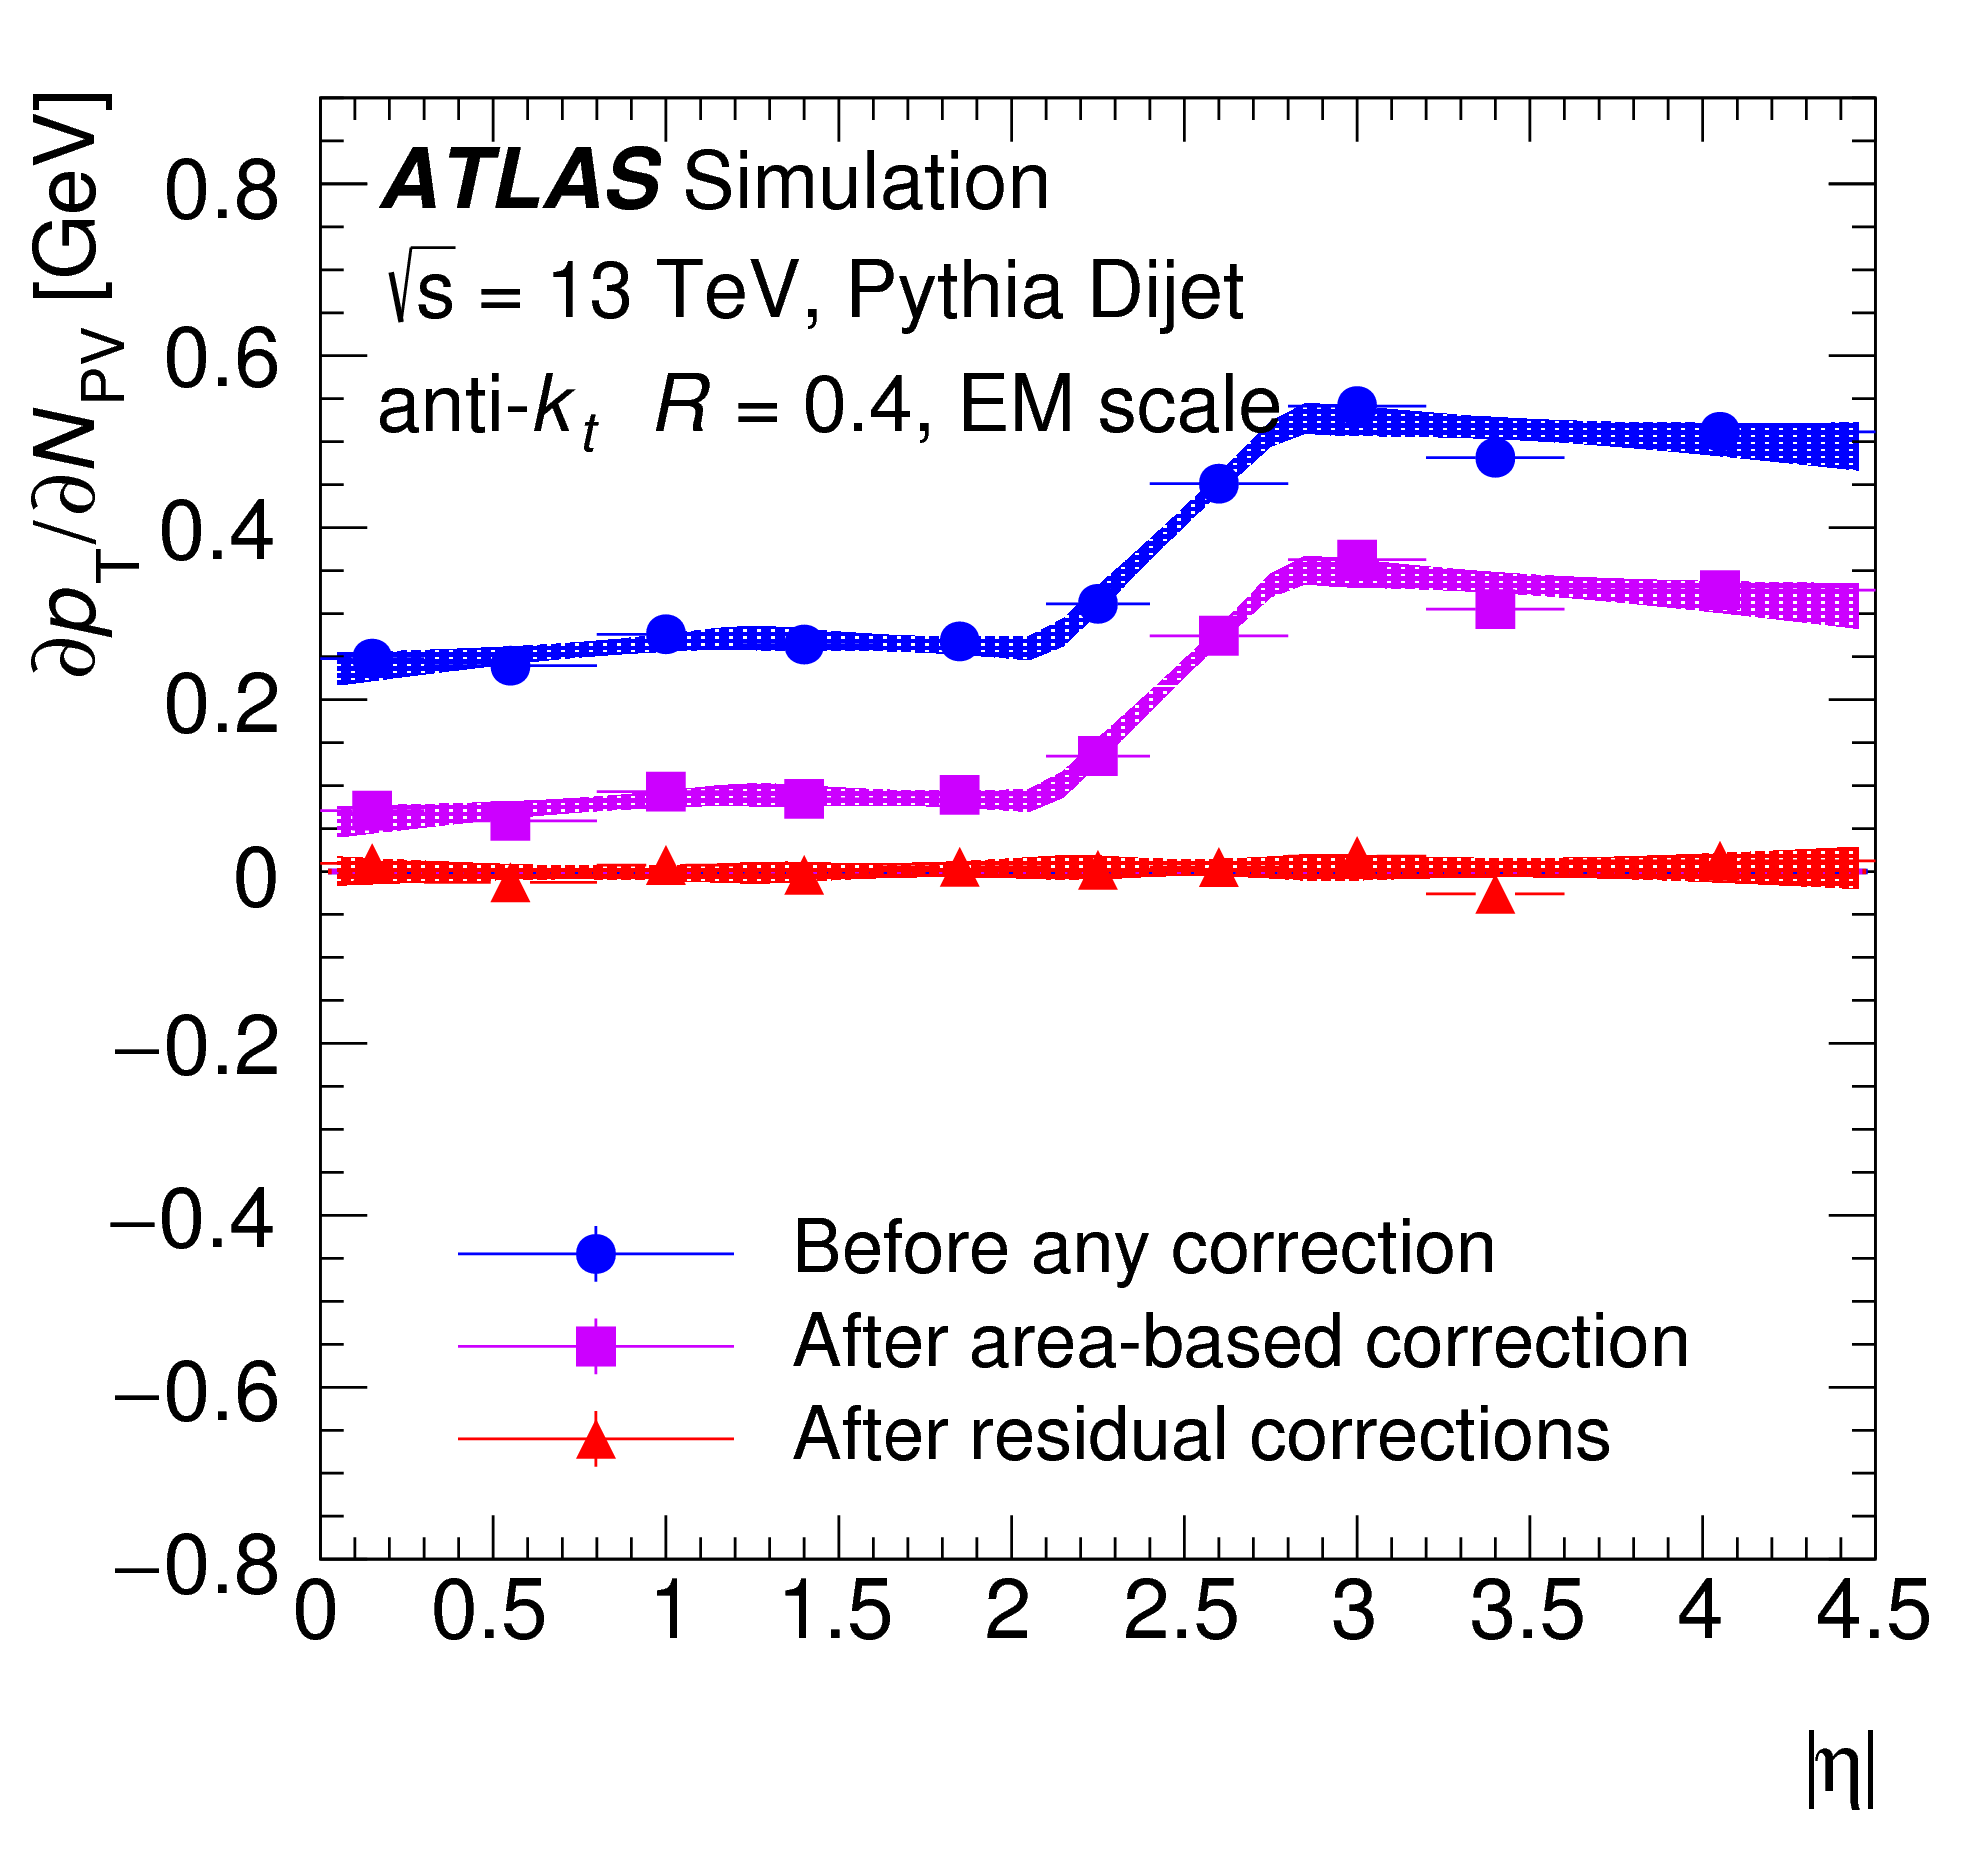
\includegraphics[width=0.4\textwidth]{figures/chapter3/jets/jet_pileup_corr_alpha}
        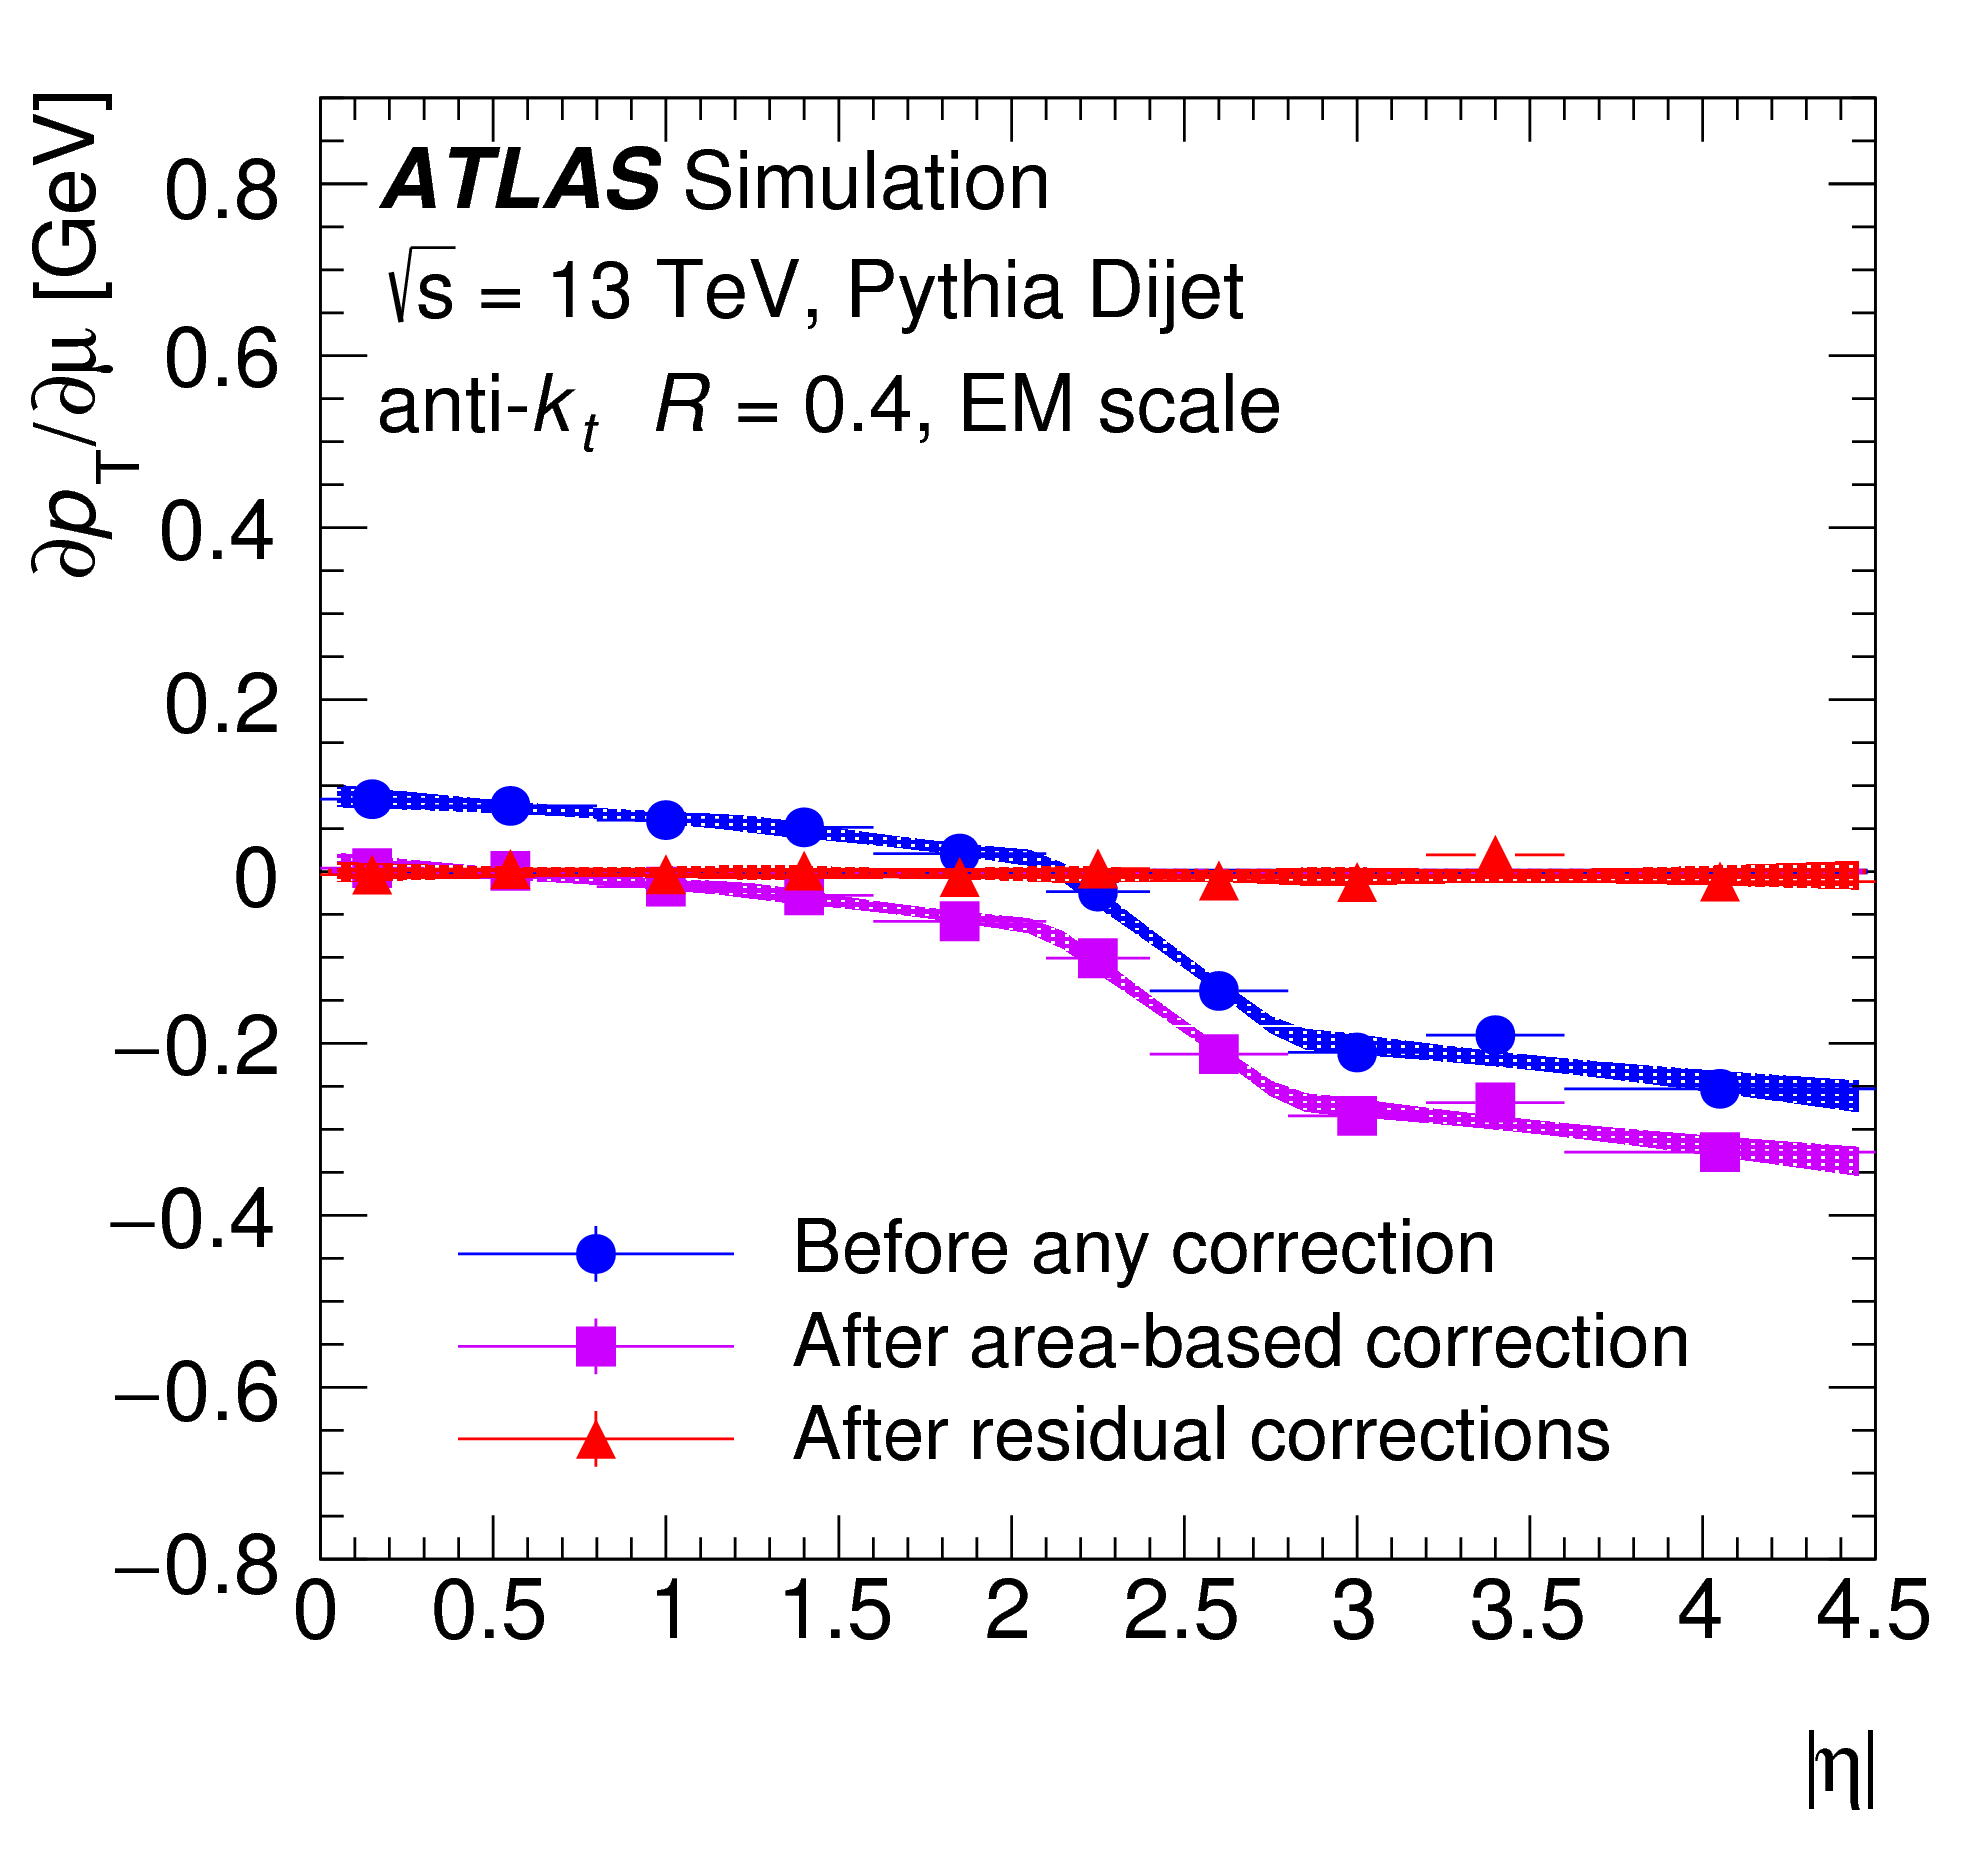
\includegraphics[width=0.4\textwidth]{figures/chapter3/jets/jet_pileup_corr_beta}
        \caption{
            Dependence of the \pT~of EM-scale reconstructed jets on \npv (in-time pileup) (\textit{left}) and on
            $\mu$ (out-of-time pileup) (\textit{right}).
            The blue curves show the dependence prior to any pileup corrections,
            the purple curves are after the area-based correction,
            and the red curves are the final dependence after the full pileup correction described in Equation~\ref{eq:jet_pileup_corr}
            is taken into account.
            Figures taken from Ref.~\cite{Aaboud:2017jcu}.
        }
        \label{fig:jet_pileup_corr}
    \end{center}
\end{figure}
